\clearpage
\section{Impact of FPF DIS data on nuclear PDFs}
\label{app:nPDF_impact_appendix}


%%%%%%%%%%%%%%%%%%%%%%%%%%%%%%%%%%%%%%%%%%%%%%%%%%%%%%%%%%%%%%%%%%%%%%%%
\begin{figure}[t]
\centering
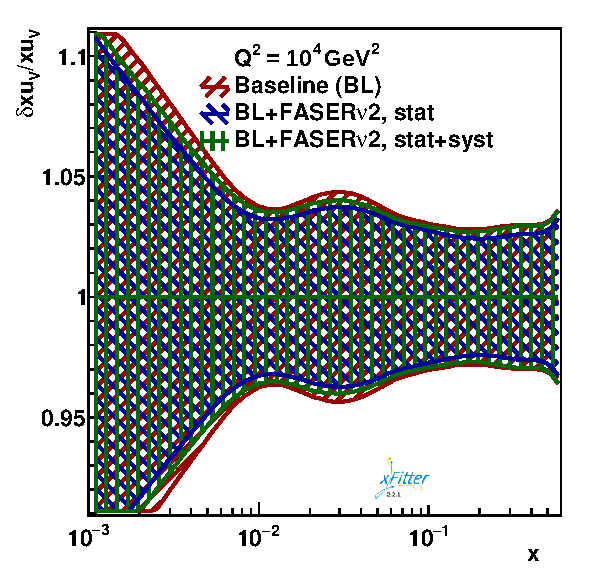
\includegraphics[width=0.32\textwidth]{plots/nuclear_fasernu2/inclusive+charm_chargediscrimination/fred05fcorr05_FASERv2_q2_10000_pdf_uv_ratio.pdf}
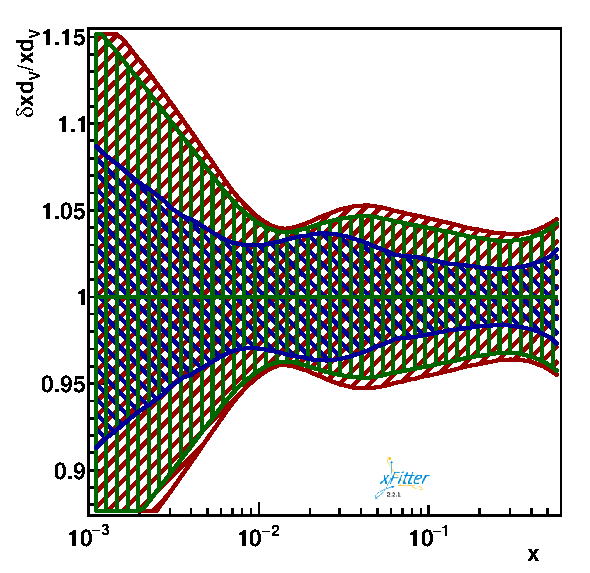
\includegraphics[width=0.32\textwidth]{plots/nuclear_fasernu2/inclusive+charm_chargediscrimination/fred05fcorr05_FASERv2_q2_10000_pdf_dv_ratio.pdf}
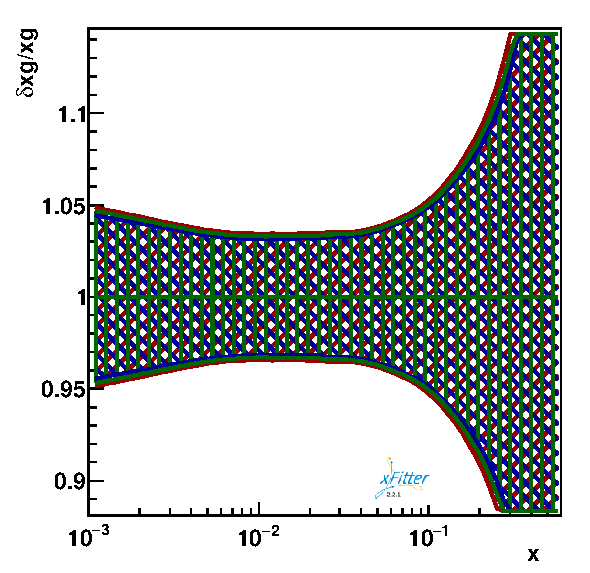
\includegraphics[width=0.32\textwidth]{plots/nuclear_fasernu2/inclusive+charm_chargediscrimination/fred05fcorr05_FASERv2_q2_10000_pdf_g_ratio.pdf}\\
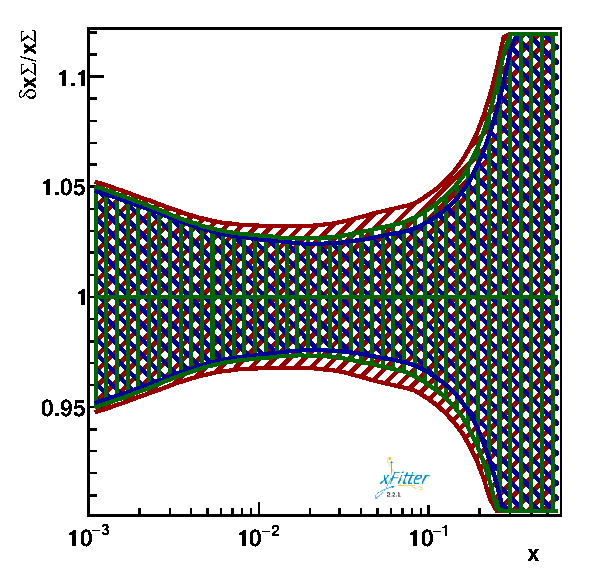
\includegraphics[width=0.32\textwidth]{plots/nuclear_fasernu2/inclusive+charm_chargediscrimination/fred05fcorr05_FASERv2_q2_10000_pdf_Sea_ratio.pdf}
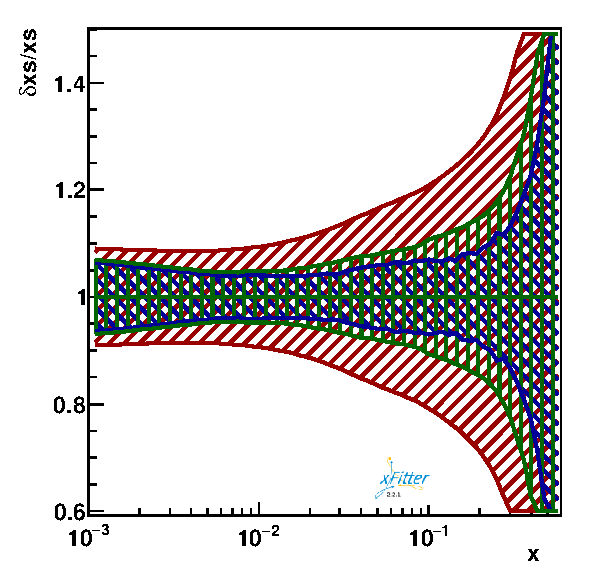
\includegraphics[width=0.32\textwidth]{plots/nuclear_fasernu2/inclusive+charm_chargediscrimination/fred05fcorr05_FASERv2_q2_10000_pdf_s_ratio.pdf}
\caption{The fractional uncertainties (68\% confidence level) at $Q^2 = 10^4 \, \textrm{GeV}^2$ of the EPPS21 global determination of nuclear PDFs (red),
specifically of the set with $A=184$ (tungsten target), 
compared to the results of profiling with the FASER$\nu$2 DIS projections.
The impact of the baseline LHC neutrino dataset, 
consisting of the FASER$\nu$2 experiment inclusive and charm structure functions and charge flavour separation,
assuming statistical errors only (blue), 
is compared to the case accounting for both statistical and systematic uncertainties (green).
}
\label{fig:profiling_syst_nuclear}
\end{figure}
%%%%%%%%%%%%%%%%%%%%%%%%%%%%%%%%%%%%%%%%%%%%%%%%%%%%%%%%%%%%%%%%%%%%%%%%
%%%%%%%%%%%%%%%%%%%%%%%%%%%%%%%%%%%%%%%%%%%%%%%%%%%%%%%%%%%%%%%%%%%%%%%%
\begin{figure}[t]
\centering
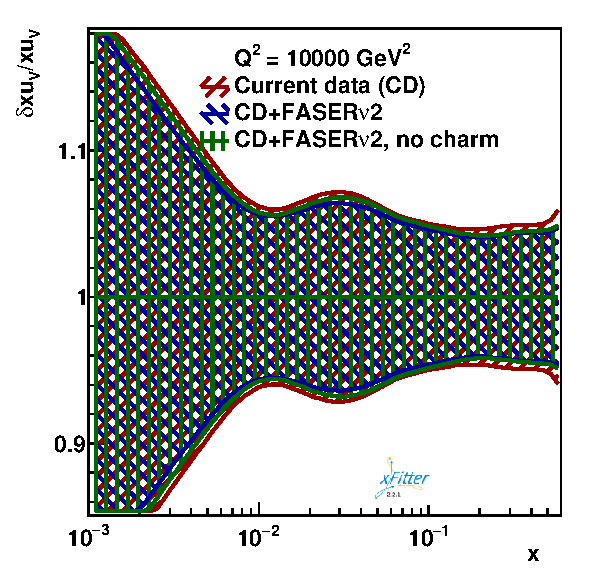
\includegraphics[width=0.32\textwidth]{plots/nuclear_fasernu2/inclusive-only_vs_inclusive+charm/statOnly_FASERv2_q2_10000_pdf_uv_ratio.pdf}
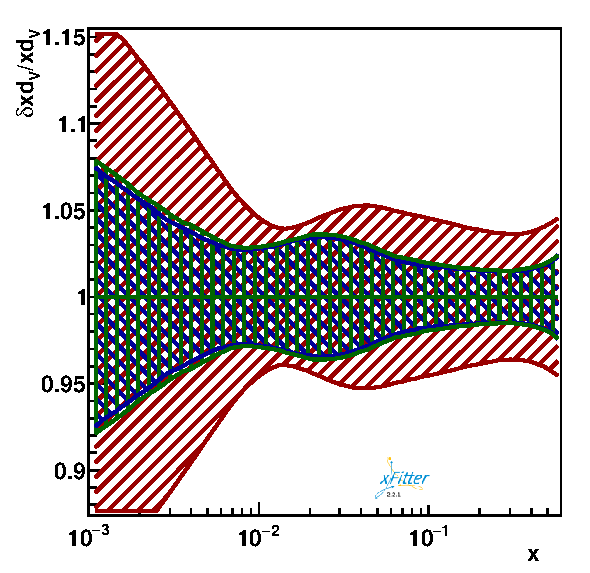
\includegraphics[width=0.32\textwidth]{plots/nuclear_fasernu2/inclusive-only_vs_inclusive+charm/statOnly_FASERv2_q2_10000_pdf_dv_ratio.pdf}
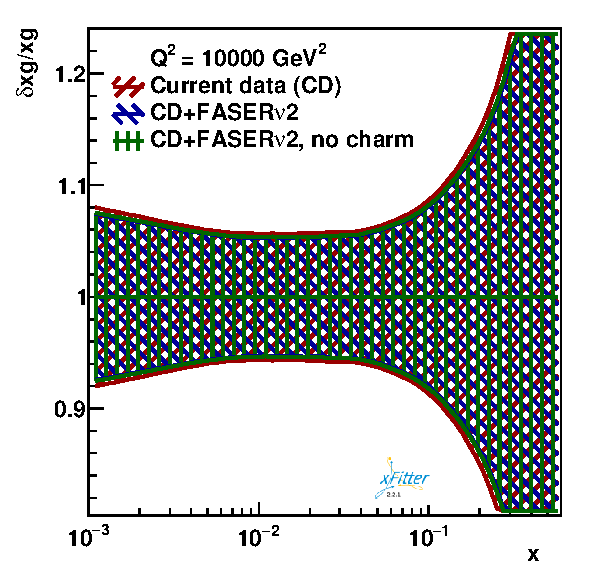
\includegraphics[width=0.32\textwidth]{plots/nuclear_fasernu2/inclusive-only_vs_inclusive+charm/statOnly_FASERv2_q2_10000_pdf_g_ratio.pdf}\\
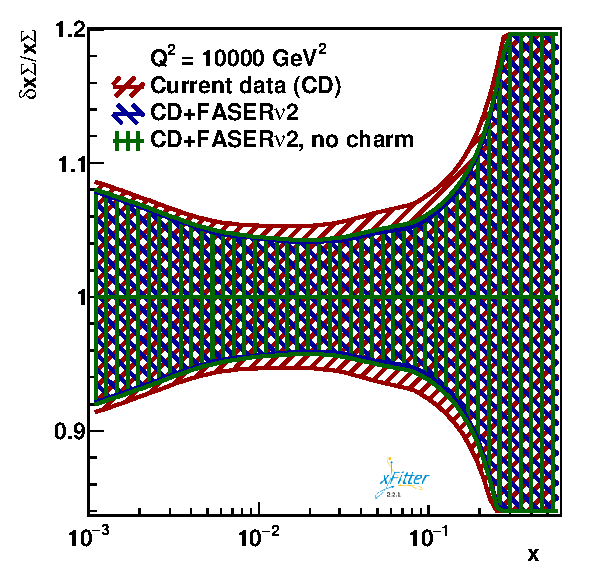
\includegraphics[width=0.32\textwidth]{plots/nuclear_fasernu2/inclusive-only_vs_inclusive+charm/statOnly_FASERv2_q2_10000_pdf_Sea_ratio.pdf}
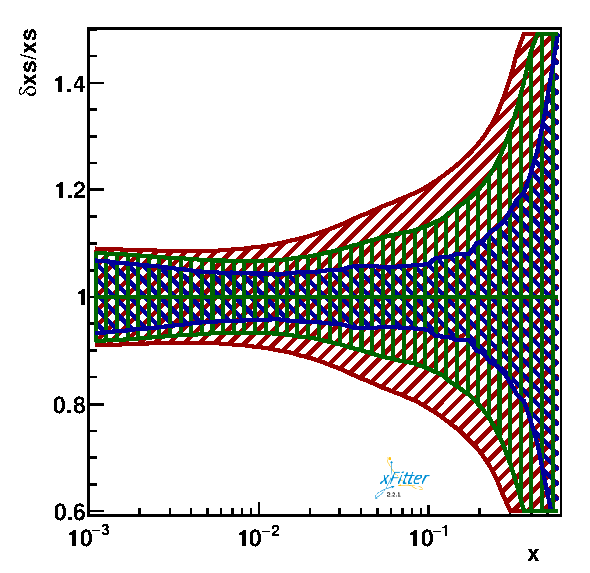
\includegraphics[width=0.32\textwidth]{plots/nuclear_fasernu2/inclusive-only_vs_inclusive+charm/statOnly_FASERv2_q2_10000_pdf_s_ratio.pdf}
\caption{The effect of FASER$\nu$2 structure functions once charm-tagged measurements are removed, assuming only statistical uncertainties in both cases.
}
\label{fig:profiling_charm_nuclear}
\end{figure}
%%%%%%%%%%%%%%%%%%%%%%%%%%%%%%%%%%%%%%%%%%%%%%%%%%%%%%%%%%%%%%%%%%%%%%%%
%%%%%%%%%%%%%%%%%%%%%%%%%%%%%%%%%%%%%%%%%%%%%%%%%%%%%%%%%%%%%%%%%%%%%%%%
\begin{figure}[t]
\centering
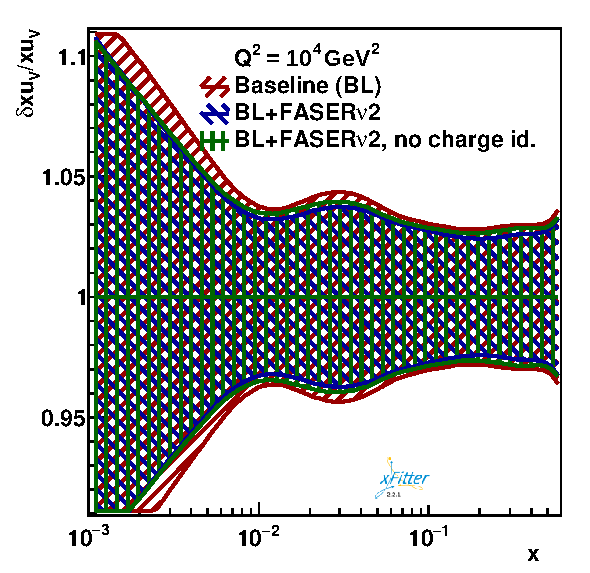
\includegraphics[width=0.32\textwidth]{plots/nuclear_fasernu2/nochargediscrimination/statOnly_FASERv2_q2_10000_pdf_uv_ratio.pdf}
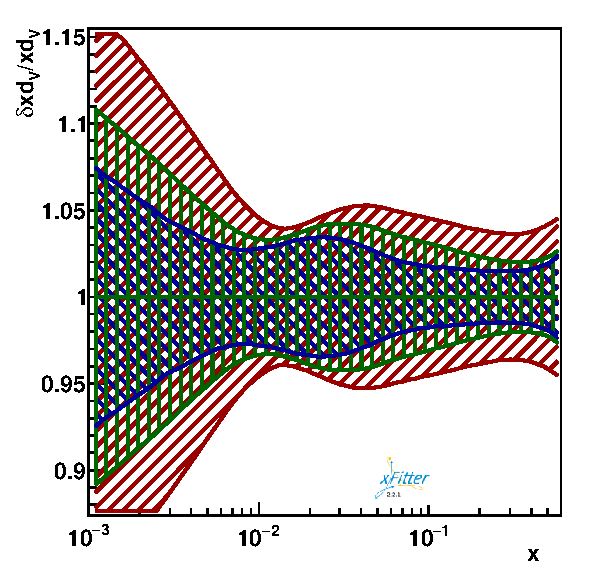
\includegraphics[width=0.32\textwidth]{plots/nuclear_fasernu2/nochargediscrimination/statOnly_FASERv2_q2_10000_pdf_dv_ratio.pdf}
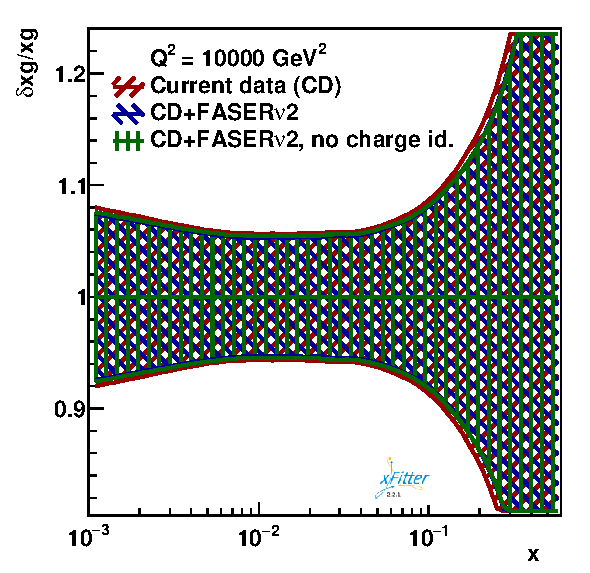
\includegraphics[width=0.32\textwidth]{plots/nuclear_fasernu2/nochargediscrimination/statOnly_FASERv2_q2_10000_pdf_g_ratio.pdf}\\
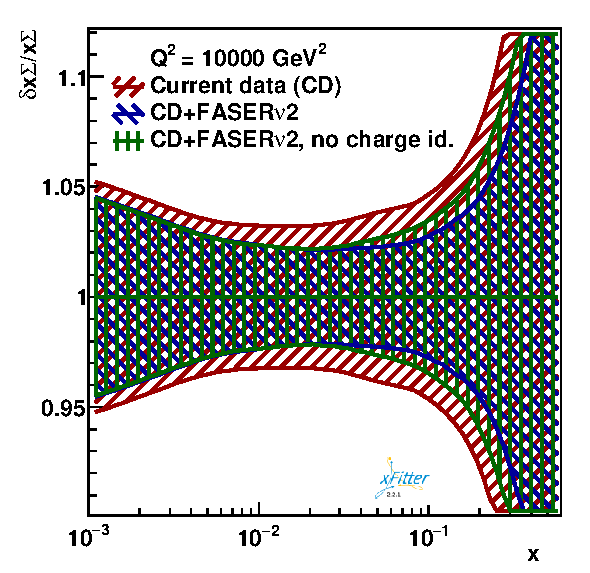
\includegraphics[width=0.32\textwidth]{plots/nuclear_fasernu2/nochargediscrimination/statOnly_FASERv2_q2_10000_pdf_Sea_ratio.pdf}
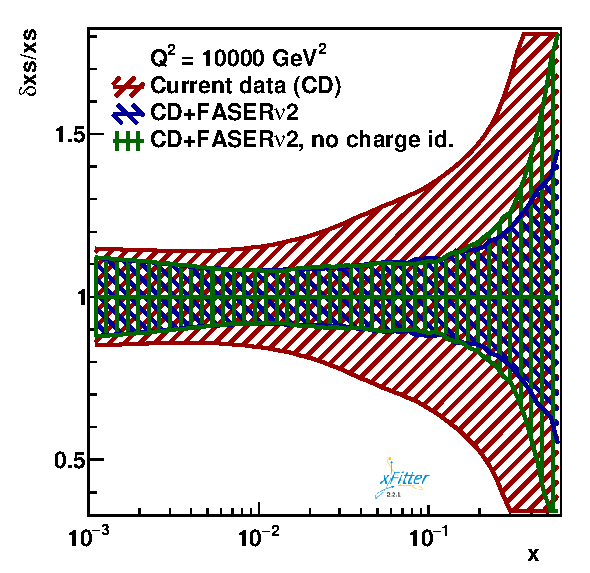
\includegraphics[width=0.32\textwidth]{plots/nuclear_fasernu2/nochargediscrimination/statOnly_FASERv2_q2_10000_pdf_s_ratio.pdf}
\caption{The effect of being unable to identify the charge of the outgoing lepton in the FASER$\nu$2 pseudodata, assuming only statistical uncertainties.
}
\label{fig:profiling_nochargediscrimination_nuclear}
\end{figure}
%%%%%%%%%%%%%%%%%%%%%%%%%%%%%%%%%%%%%%%%%%%%%%%%%%%%%%%%%%%%%%%%%%%%%%%%


